% =============================================================================
% 3. ANALISIS EXPLORATORIO DE DATOS
% =============================================================================
\section{An\'alisis exploratorio}
\label{sec:exploratory-analysis}

\subsection{Distribuci\'on de patolog\'ias}

El an\'alisis de prevalencia revel\'o un desbalance significativo entre clases (Figura~\ref{fig:prevalence}): Pleural Effusion presenta la mayor prevalencia ($\sim$40\%), seguida de Atelectasis ($\sim$30\%), Cardiomegaly ($\sim$15\%), Edema ($\sim$12\%) y Consolidation ($\sim$5\%). Este desbalance justifica el uso de AUC-ROC como m\'etrica principal, ya que es insensible al umbral de decisi\'on y al desbalance de clases---criterio adoptado por la competencia oficial CheXpert \cite{irvin2019chexpert}.

\begin{figure}[H]
    \centering
    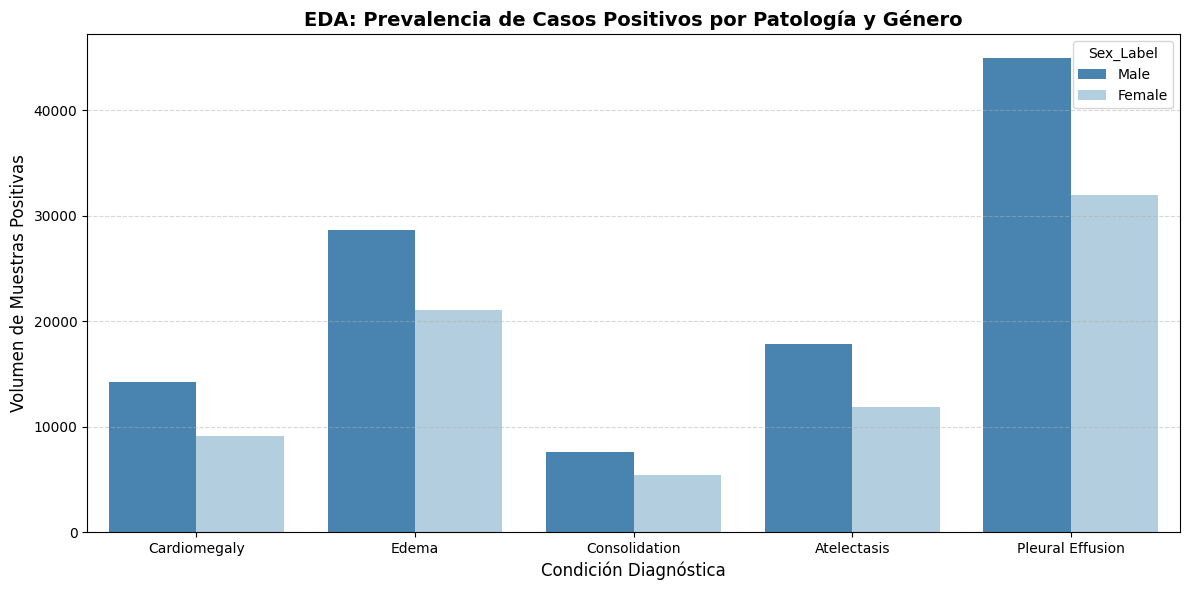
\includegraphics[width=\columnwidth]{figures/pathology-prevalence-by-gender.png}
    \caption{Prevalencia de casos positivos por patolog\'ia y g\'enero en el conjunto de entrenamiento ($\sim$190k im\'agenes frontales).}
    \label{fig:prevalence}
\end{figure}

La co-ocurrencia de patolog\'ias (un paciente puede presentar m\'ultiples condiciones simult\'aneamente) justifica la elecci\'on de clasificaci\'on multi-etiqueta con activaci\'on Sigmoid independiente por clase, en lugar de Softmax excluyente.

\subsection{An\'alisis estad\'istico: variable sexo}

La composici\'on demogr\'afica del dataset muestra un ratio Male/Female de 1.42:1 (112,151 hombres vs 78,875 mujeres), consistente con la poblaci\'on hospitalaria de Stanford. Para determinar si el sexo biol\'ogico deb\'ia incluirse como predictor, se realiz\'o un an\'alisis de independencia mediante test Chi-cuadrado y tama\~no del efecto (V de Cram\'er) para cada patolog\'ia (Tabla~\ref{tab:chi2}).

\begin{table}[H]
\centering
\caption{An\'alisis de independencia entre sexo y patolog\'ia.}
\label{tab:chi2}
\small
\begin{tabular}{lccc}
\toprule
\textbf{Patolog\'ia} & \textbf{p-value} & \textbf{V de Cram\'er} & \textbf{Efecto} \\
\midrule
Cardiomegaly     & $<$ 0.05 & 0.06 & Negligible \\
Edema            & $<$ 0.05 & 0.04 & Negligible \\
Consolidation    & $<$ 0.05 & 0.02 & Negligible \\
Atelectasis      & $<$ 0.05 & 0.03 & Negligible \\
Pleural Effusion & $<$ 0.05 & 0.05 & Negligible \\
\bottomrule
\end{tabular}
\end{table}

Con $N > 200{,}000$ muestras, la significancia estad\'istica ($p < 0.05$) no implica significancia pr\'actica. Los valores de V de Cram\'er ($< 0.1$) confirman que el sexo explica menos del 1\% de la varianza en la presencia de patolog\'ias.

\subsection{Decisi\'on: exclusi\'on de la variable sexo}

Se decidi\'o excluir la variable sexo del modelo por cuatro razones fundamentales:

\begin{enumerate}
    \item \textbf{Efecto pr\'actico negligible}: V de Cram\'er $< 0.1$ para todas las patolog\'ias.
    \item \textbf{Riesgo de sesgo algor\'itmico}: incluir el sexo puede perpetuar disparidades diagn\'osticas. \cite{seyyedkalantari2021bias} demostraron que modelos entrenados en CheXpert subdiagnostican sistem\'aticamente a pacientes femeninas incluso sin sexo como input.
    \item \textbf{Redundancia}: \cite{jabbour2020shortcuts} y \cite{gichoya2022ai} demostraron que las CNNs pueden predecir sexo desde la imagen sola con AUC $>$ 0.96, lo que indica que la red ya tiene acceso impl\'icito a esta informaci\'on a trav\'es de marcadores anat\'omicos.
    \item \textbf{Simplicidad}: un modelo solo-imagen es m\'as f\'acil de desplegar en producci\'on y no requiere metadatos cl\'inicos del paciente.
\end{enumerate}

Esta decisi\'on se alinea con la recomendaci\'on de \cite{larrazabal2020gender}, quienes demostraron que el desbalance de g\'enero en datasets de CXR produce clasificadores sesgados independientemente de incluir sexo como variable. La limitaci\'on reconocida es que excluir la variable no elimina el sesgo---solo impide medirlo directamente---por lo que se implement\'o una auditor\'ia de equidad desagregada por sexo en la fase de evaluaci\'on (Secci\'on~\ref{sec:ethics}).

\begin{figure}[H]
    \centering
    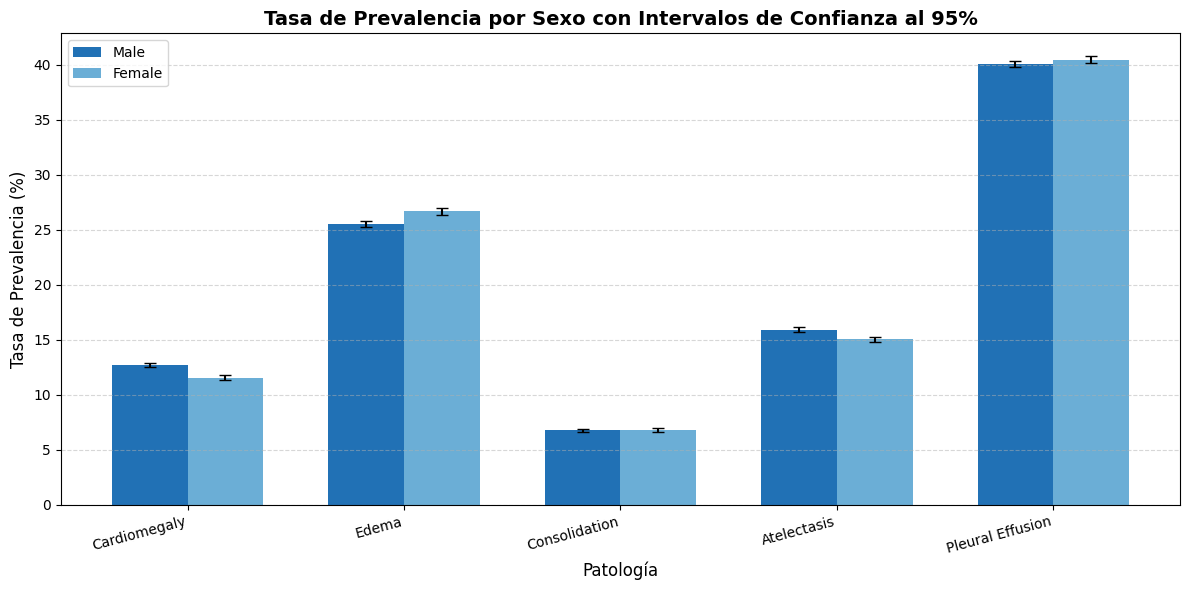
\includegraphics[width=\columnwidth]{figures/prevalence-rate-by-sex-ci95.png}
    \caption{Tasa de prevalencia por sexo con intervalos de confianza al 95\%. Las diferencias son estad\'isticamente significativas pero pr\'acticamente negligibles (V de Cram\'er $<$ 0.1).}
    \label{fig:prevalence-sex}
\end{figure}
